%%%%%%%%%%%%%%%%%%%%%%%%%%%%%%%%%%%%%%%%%
% Structured General Purpose Assignment
% LaTeX Template
%
% This template has been downloaded from:
% http://www.latextemplates.com
%
% Original author:
% Ted Pavlic (http://www.tedpavlic.com)
%
% Note:
% The \lipsum[#] commands throughout this template generate dummy text
% to fill the template out. These commands should all be removed when 
% writing assignment content.
%
%%%%%%%%%%%%%%%%%%%%%%%%%%%%%%%%%%%%%%%%%

%----------------------------------------------------------------------------------------
% PACKAGES AND OTHER DOCUMENT CONFIGURATIONS
%----------------------------------------------------------------------------------------

\documentclass[12pt]{article}

\usepackage{fancyhdr} % Required for custom headers
\usepackage{lastpage} % Required to determine the last page for the footer
\usepackage{extramarks} % Required for headers and footers
\usepackage{graphicx} % Required to insert images
\usepackage{lipsum} % Used for inserting dummy 'Lorem ipsum' text into the template
\usepackage{wrapfig}
\usepackage{enumitem}
\usepackage{subcaption}
\usepackage{color}

\usepackage[explicit]{titlesec}

\usepackage[export]{adjustbox}

% Margins
\topmargin=0in
\evensidemargin=0in
\oddsidemargin=0in
\textwidth=6.5in
\textheight=9in
\headsep=0.5em 

\linespread{1} % Line spacing

% list spacing
\setlist{nosep}

% caption spacing
% \setlength\belowcaptionskip{-3pt}

% \bibliographystyle{plain}

\titleformat{\section}
  {\bfseries}{\thesection}{0em}{#1}
\titlespacing*{\section}{0em}{0em}{0em}[0em]

% Set up the header and footer
\pagestyle{fancy}
\lhead{\AuthorName} % Top left header
\chead{\Title} % Top center header
\rhead{\Subject} % Top right header
\fancyfoot{}
% \lfoot{\lastxmark} % Bottom left footer
% \cfoot{} % Bottom center footer
\rfoot{Page\ \thepage\ of\ \pageref{LastPage}} % Bottom right footer
\renewcommand\headrulewidth{0.4pt} % Size of the header rule
% \renewcommand\footrulewidth{0.4pt} % Size of the footer rule

\setlength{\parskip}{0.3em}
\setlength\parindent{10pt} % Removes all indentation from paragraphs


\newcommand{\Title}{Project Narrative} % Assignment title
\newcommand{\Subject}{NSTRF 2016}
\newcommand{\AuthorName}{Colin Rennie} % Your name
\newcommand{\kostas}[1]{{\color{blue} #1}}

\begin{document}
\newpage

\begin{center}
{\bf Coordinated Planning and Control for \\ Tethered Robot Pairs }

\end{center}
\vspace{-.1in}

%---------------- Introduction ------------------
%Tethered Robot Importance 
%Planetary exploration
%Situations needing tethers for science targets
%Communications

\noindent {\bf Motivation:} Many important and rewarding science
target locations on extra-planetary bodies lie in terrain that is
rocky, uneven, or involves traversing steep inclines. Consider the
search for ice in underground caves on Mars, or collecting soil
samples and images from the bottom of a crater or ravine.  These
tasks, while very rewarding in terms of scientific value, are not
easily achieved by humans nor the current generation of planetary
rovers. This shortcoming of current exploratory technology has spurred
considerable interest in the development of next generation rover
designs featuring a tether that either connects the rover to a static
point in the environment \cite{axel_planning, dante_results, 
dante_design} or, even more
desirably, connects to another rover vehicle of equal capability. A
tethered team of space exploration rovers benefits from the stability
that a tether can provide while rappelling down difficult terrains. 
The team is also 
able to reconfigure to provide maximal stability to the actively 
descending rover. Furthermore, robots can swap roles between (1)
providing stability to their counterparts and (2) traversing the terrain,
depending on sensing input. These benefits allow a tethered team to safely
traverse difficult terrain well beyond what a single anchored robot
could achieve.

\begin{wrapfigure}{r}{0.5\textwidth}
  % \begin{center}
  \vspace{-0.2in}
  \begin{subfigure}{.26\textwidth}
    \centering
    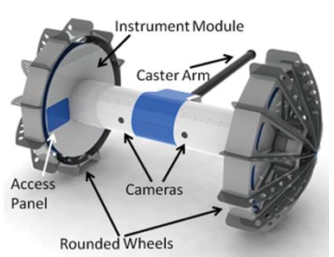
\includegraphics[width=.75\linewidth]{axel_prototype}
    \caption{}
    \label{fig:axel}
  \end{subfigure}%
  \begin{subfigure}{.23\textwidth}
    \centering
    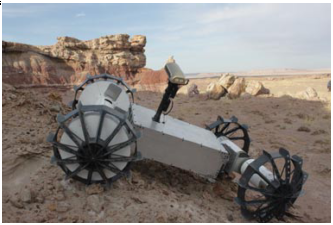
\includegraphics[width=.95\linewidth]{duaxel_prototype}
    \caption{}
    \label{fig:duaxel}
  \end{subfigure}
  \begin{subfigure}{.245\textwidth}
    \centering
    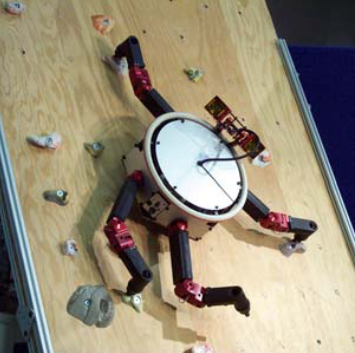
\includegraphics[width=.88\linewidth]{lemur_prototype}
    \caption{}
    \label{fig:lemur}
  \end{subfigure}%
  \begin{subfigure}{.245\textwidth}
    \centering
    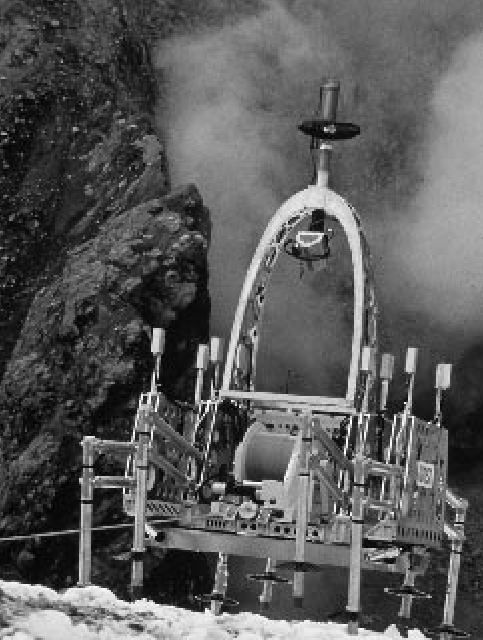
\includegraphics[width=.65\linewidth]{dante_prototype}
    \caption{}
    \label{fig:dante}
  \end{subfigure}  % \end{center}
  \label{fig:prototypes}
  \vspace{-0.1in}
  \caption{(a) The Axel II rover prototype (b) Two Axel II rovers in DuAxel configuration 
  with support structure (c) Lemur IIb autonomous climbing robot (d) Dante II robot exploring a 
  volcanic crater. Images: \cite{duaxel, lemur_design, dante_results}.}
\end{wrapfigure}

\noindent {\bf Objective:} This report proposes viable solutions for
two key and related problems for effective tethered robotic teams.
Progress in these directions can significantly improve tethered robot 
technology for
planetary exploration: (a) coordinated control for reconfiguring a
tether between a pair of rovers to deal with unforeseen terrain
challenges, where both robots actively participate in this process,
and (b) a planning framework that utilizes the control strategy as a
module for coordinated descent or ascent of difficult terrain for a
tethered robotic team.  These solutions should be general enough to
be platform-independent and apply to other space critical
applications. For example, a tethered team of Robonauts, Valkyries or
other humanoid robots could utilize such solutions during a repair
mission of the International Space Station.

%----------------------------------------------
%---------------- Background ------------------
%----------------------------------------------

{\bf\noindent Relevant Background on Tethered Rovers}

Recent research into robot designs for the traversal of harsh and
difficult terrains has featured several different designs with
alternative means of locomotion. Certain systems include an actuated
winch or spooled tether used for communication and/or stability while
locomoting.  Notable examples include an eight-legged walking robot
attached to a stationary base [Fig. \ref{fig:dante}] and a pair of
two-wheeled differential drive robots connected with a soft tether
[Fig. \ref{fig:duaxel}]. Even more novel recent robot designs could
benefit from the presence of a tether attachment to an exploratory
counterpart. This list includes Lemur IIb, a four-legged climbing
robot [Fig. \ref{fig:lemur}], which could potentially use an actuated
tether to swing its counterpart onto protruding overhangs and then, in
turn, rappel from the stabilized counterpart robot in order to reach
the overhang safely.

%Dante II (& lemur II?)

The Dante II robot design consisted of eight legs for locomotion, an actuated 
winch used for rappelling down steep and difficult terrain
from a static anchor point, and a variety of sensing equipment for data 
retrieval \cite{dante_design}.  
In 1994 the system was deployed into Mount Spurr, an active
volcanic site, in order to record data for further scientific
analysis. During the mission the robot suffered from a
failure where the robot incurred a lateral force at its contact point
with the tether, fell over, and was not able to correct itself \cite{dante_results}. Apart
from this occurrence, however, the 5-day mission was regarded as a
success in showing the capabilities of tethered robotic systems to act
as ``surrogate scientists''; exploring where humans would not
otherwise be able.

\begin{wrapfigure}{r}{0.5\textwidth}
  \vspace{-0.4in}
  \begin{subfigure}{.45\textwidth}
    \centering
    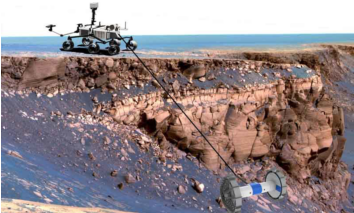
\includegraphics[width=.95\linewidth]{axel_deploy}
    \caption{}
    \label{fig:axeldeploy}
  \end{subfigure}\\
  \begin{subfigure}{.25\textwidth}
    \centering
    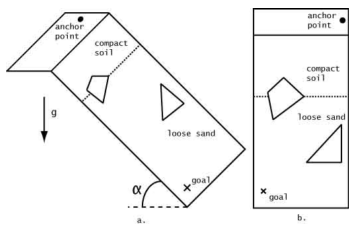
\includegraphics[width=.99\linewidth]{planar_terrain}
    \caption{}
    \label{fig:planarterrain}
  \end{subfigure}%
  \begin{subfigure}{.2\textwidth}
    \centering
    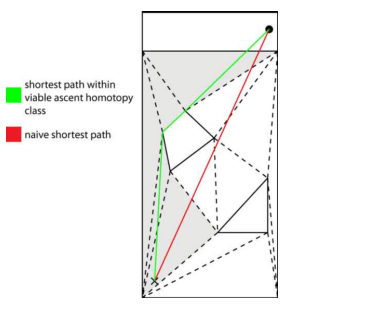
\includegraphics[width=.95\linewidth]{planar_path}
    \caption{}
    \label{fig:planarpath}
  \end{subfigure}  % \end{center}
  \label{fig:dsolution}
  \vspace{-0.1in}
  \caption{(a) Conceptualized descent terrain for Axel II mission (b) example projection of terrain to 2D plane
  (c) example solution: viable controllable regions for ascent (shaded), naive shortest path (red), shortest path within 
  viable homotopy class (green). Images: \cite{ axel_planning}. }
\end{wrapfigure}

%Axel platform (+picture)

More recently, NASA's Jet Propulsion Laboratory (JPL) has been working on a
two-wheeled differential drive tethered robot, appropriately named
``Axel''. The Axel II robot design features collapsible, paddled
wheels, making the system more appropriate for longer and more remote
missions as this design is more robust to issues such as
high-centering and failures such as that encountered by Dante II
\cite{axel_design}. Two variants of the system are
presented: one in which Axel is attached to a stationary anchor point,
and a second where two Axel robots are tethered together and deployed
via a central support beam (``DuAxel'') \cite{duaxel}.

%Motion planning solution

A key challenge in either variation was how to plan autonomous
descent and corresponding ascent paths for the deployed, tethered Axel
robot in rocky extra-planetary terrains.  A solution
framework was presented which projected this complex problem to a
two-dimensional plane. It built on foundational work addressing the
tether constraint problem from a computational geometry perspective
\cite{ties_that_bind, min_homotopies} and extended this approach to
produce ``controllable'' paths by deriving equations of motion arising
from the constraints of the Axel robot \cite{axel_planning}. The
resulting algorithm first plans the more difficult ascent path and
then uses the solution to limit its search for viable descent paths
lying in the same homotopy class.

%Problems
%   Quasi-static, no cable friction with ground assumed
%   solution is planar, over-simplifying the environment
%   assumes static anchor point (base unit)

While this solution represents substantial progress well-grounded in
foundational work, the assumptions and simplifications may limit its
applicability. In particular, projecting complex 3D terrain
environments in 2D and representing obstacles as simple polygons
[Fig. \ref{fig:planarterrain}] may be not adequate for many realistic
extra-planetary terrains.  This strategy also assumes perfect prior
knowledge of the environment, frictionless interaction of the tether
with the ground plane, and quasi-static motion of the robot.
Furthermore, it remains an open question as to how best to plan
autonomous motions for the DuAxel configuration where two dynamic
robots take turns belaying each other.

% \kostas{it seems to me that you are not describing any of the (non-NASA)
%   references that I forwarded you about planning for tethered robots -
% you didn't find them useful?}

%-----------------------------------------------------
%---------------- Proposed Research ------------------
%-----------------------------------------------------

% Doing so allows us to plan in a 
% kinodynamic way (taking into account constraints on velocity and acceleration of the robot) and generate solutions which 
% account for the robot's dynamics (as opposed to quasi-static solutions)

{\bf\noindent Proposed Research}

{\sl The main goal of this research is to address the problem of
  planning for tethered teams of exploratory robots, while considering
  the complexities that arise from realistic three-dimensional
  terrains.  The proposed solution first considers a control strategy
  for addressing unforeseen obstacles and failures. It then uses this
  strategy as a module in planning paths for tethered robotic teams,
  in which the robots alternate between exploring and providing
  support to their counterparts.}

The following discussion will focus on the case of a tethered pair of
robots but can be generalized to larger teams. The high-level approach
is applicable to varying types of tethered rovers provided that they
have a means of: (1) actuating the tether at its contact points with
each rover, and (2) measuring the forces exerted on each rover at the
tether's contact points. The most similar existing system which could
utilize such solutions is the DuAxel rover design, which fits these
specifications already. Nevertheless, one can also apply this approach
to a pair of Lemur IIb robots free-climbing a vertical and jagged
cliff face or even a pair of traditional wheeled rovers descending a
steep and rocky mountainside. Moreover, exciting future extensions of this 
work include the extension of this work to larger (either in number of 
rovers per team, or number of tethered pairs) teams of tethered rovers.  

%TABS Roadmap applicability
As this proposal is developed with the overall goal of providing more robust and 
capable algorithms for extra-planetary exploration, we believe it has primary 
applicability to the technology goals of TABS 4.5.7 (and relatedly, TABS 4.2.6). 
An inextricable portion of the proposed technology also aims to progress 
research in multi-agent coordination. As such, we believe there is a strong 
connection with the technology goals of TABS 4.5.4 as well.  

%---------------- Research Problem 1 ------------------

\noindent\underline{Research Problem 1: Coordinated control of a soft tether}

{\sl Goal: In presence of imperfect terrain information, we require a
  strategy for dealing with both unforeseen obstacles and unplanned
  tether entanglements on rocky terrain elements. }

% Outline the problems

In the following, we consider several potentially difficult situations
that are likely to arise when planning for a tethered robotic pair
under imperfect information about the terrain. In addressing this
problem in the full 3D workspace, a strategy is required which can
deal with two important potential failure cases. First, while an
exploratory rover is moving along its planned obstacle-free path, the
tether comes in contact with and becomes entangled on uneven terrain
(the ``snagging'' case). Second, while performing the exploratory
role, a rover encounters an unknown obstacle obstructing its planned
path, which we'll call the ``reevaluation'' case (addressed in the
planar case in previous, related work \cite{axel_online}).

% reevaluation case

In the ``snagging'' case [Fig. \ref{fig:tethersnag}], we propose to
develop a low-level control law capable of inducing a traveling wave
in the tether by employing an oscillatory control policy at the
actuated tether contact of the rover closest to the tether snag
location. This approach is similar to the strategy used by humans when
they encounter the same situation while mountain climbing.  The
challenge in this strategy, however, is that once the tether is free,
it's likely to impart a substantial force on the robot's stabilizing
counterpart, potentially resulting in dangerous jerking in a partially
known environment.  A promising solution to this problem would be to
induce in response a counteracting wave from the stabilizing rover's
actuated tether contact. To this end, the first direction to explore
involves building a model (potentially analytically) of the expected
forces exerted by the induced wave on the counterpart robot.  We would
then use this model in the context of a model predictive control
approach, where the low-level control policy optimizes its current
control with respect to counteracting the incurred force over a finite
time horizon of future predictions. The second direction involves
exploring model-free approaches (e.g., designing an admittance
controller), as it's possible that reacting to forces incurred is a
more feasible solution than accurately predicting them ahead of time.

% integration case: online re-planning wrt coordination between avoidance control and motion planning algo
\begin{wrapfigure}{r}{0.5\textwidth}
  \begin{center}
    \vspace{-0.3in}
    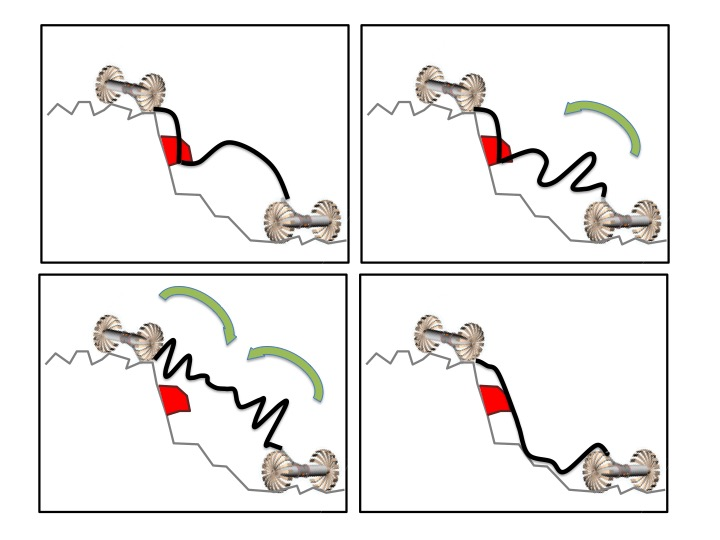
\includegraphics[width=0.48\textwidth, right]{tether_desnag.jpg}
  \end{center}
  \vspace{-0.4in}
  \caption{During a coordinated descent down a rocky extra-planetary
    surface, the tethered rover pair encounters an unplanned snag of
    the tether with a rock in the terrain (red). The situation is
    resolved by using the coordinated wave-inducing control strategy
    (green arrows indicate controls applied) to free the tether.}
  \label{fig:tethersnag}
\end{wrapfigure}

In the ``reevaluation'' case of encountering an unmodeled obstacle in our
path, what we must first decide is whether or not we can configure our
tether such that we are able to place the tether in an arbitrary
configuration on either side of the obstacle once we have moved past
it. The reason being that
while the unmodeled obstacle may not cause significant problems for
our current rover's descent, planning the current stabilizing rover's
traversal of the same slope is much more constrained as it does not
have a stabilizing tether. Being able to place the tether on either
side of the obstacle would then allow us to first plan the descent of
the current stabilizing rover (incorporating this new obstacle), and
then use the traversing rover to place the tether on the side of the
obstacle that is easiest for the stabilizing rover to traverse.

There are two tools available to determine whether this new obstacle
is surmountable. By considering the height of the obstacle, we can
search for configurations of the tethered pair which raise the tether
above the obstacle.  Alternatively, it is possible to extend the
snagging strategy outlined above -- simulating the effects of various
parameterizations of our wave-inducing control policies to find one
that would be able to surmount the obstacle. If such a policy is
found, then it can be combined with a motion plan to move the
exploratory rover to the desired side of the new obstacle, terminating
the control policy once it has successfully reached the target state.

%---------------- Research Problem 2 ------------------

\noindent\underline{Research Problem 2: Motion planning for dynamic
  tethered rover pairs }

{\sl Goal: Develop a robust motion planning framework for a tethered
  team of rovers by integrating the control strategy outlined above as
  a subroutine in cases of environmental obstacles and tether
  entanglements. This framework can plan the coordinated traversal of
  difficult terrain while the rovers alternate exploratory and
  stabilizing roles. }

%Making use of the control strategy presented above when faced with
%unforeseen obstacles and situations, we can now outline our strategy
%for robustly solving the motion planning problem of the coordinated
%traversal (ascent or descent) of difficult and partially known
%extra-planetary terrain.

Given incomplete knowledge of the environment, the proposed strategy
is to first select a set of maximally stable waypoints throughout the
terrain. It is then possible to proceed iteratively and in an
alternating fashion, first planning the descent of one of the rover
pair to the first stable waypoint, then the other to some next stable
waypoint closer to the goal. The waypoints can then be thought of as
``role reversal'' locations. When unforeseen obstacles (or snags) are
encountered, the planning strategy can call upon the control strategy
as a module and then re-plan.  Importantly, re-planning under this
strategy only requires re-computing the path between the current set
of waypoints, as opposed to the trajectory of the entire traversal.

\begin{wrapfigure}{r}{0.5\textwidth}
  \begin{center}
  \vspace{-0.4in} 
  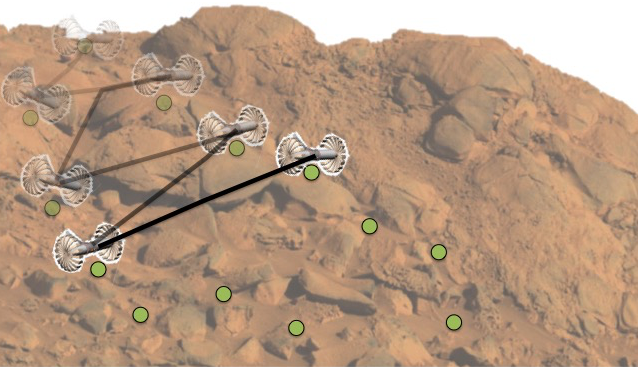
\includegraphics[width=0.48\textwidth, left]{descent_2.png}
  \end{center}
  \vspace{-0.2in}
  \label{fig:descent}
  \caption{Conceptualized time lapse of coordinated descent of a tethered robot pair. Tether shown in black, computed 
  waypoints in green.} \vspace{-.2in}
\end{wrapfigure}
%Solution Sampling-based

Planning between two waypoints in the full 3D workspace and taking
into account the dynamics of the tethered systems can be addressed by
using a variety of trajectory-based methods. One promising solution
corresponds to sampling-based motion planners, which have been
successfully applied to solve similarly high-dimensional problems with
complex kinematic and dynamic constraints \cite{zak_kino}. A typical
limitation with these methods, however, is the relatively high
computation requirements to sample enough states to converge to a
high-quality solution. Considering that the objective is to
dynamically replan so as to respond to sensing input, an objective of
this work is to decrease the amount of time required to find solutions
while still addressing this problem in the full state space of the
underlying robotic system.

%Solution 

Several techniques can be drawn upon for this purpose. The first set
of approaches involve biasing the sampling of states in ways that
utilize key aspects of this specific challenge. For example, by
computing the ``most stable'' support position of the stabilizing
rover (i.e., perpendicular to the current position of the exploratory
rover) and biasing the sampling process toward the subset of the state
space with this property. 

This work will explore whether or not it
is effective to project the problem from the full state space, which
may be very high-dimensional, depending on the degrees of freedom of
the involved robots, to appropriate lower-dimensional task space
projections. For example, the problem may potentially be dissected 
into multiple subproblem
manifolds, where it may be possible to achieve reliable solutions much
faster than in the full state space. In certain cases, this has been
achieved through use of machine learning techniques, where it is
possible to train a model to learn the important sub-manifolds of a
particular system's state space while also learning to predict which
static configurations for other state dimensions would be most
effective for solving the complete problem \cite{learning_biases}.


% \kostas {
%   {\bf Beyond these research problems:}
%   Describe how you can go from a pair of robots to multiple robots and
%   how this could also be applied to the case of a robot-human team
%   (additional complexities in this case). 
% }
{\bf\noindent Visiting Technologist Experience}

In making progress toward the stated objectives of this research, hands-on experience with NASA 
engineers at a NASA research center would be invaluable. Observing and interacting with the most promising 
rover prototypes currently in development would allow my efforts in modeling these systems to be as accurate 
and share as many traits as possible. Working with the mechanical engineers building these systems would 
allow me crucial insight into the capabilities and limitations of current prototypes and would promote 
faster dissemination of inter-disciplinary ideas. Beyond benefits directly to the research, these experiences 
would be tremendously beneficial to my own education as a scientist. 

Many of the systems (Axel II, DuAxel, Lemur IIb) mentioned in this paper were developed and tested at NASA 
JPL, which would make this location an ideal candidate for visiting experience. However, as the ideas presented here 
are largely independent of the platform, I believe it could also be beneficial to work with systems and 
engineers at NASA Ames (Tensegrity robots, KRex) or Johnson Space Center (Robonaut 2).


% ----------------end of document body---------------------

%---------------- start of references------------------
\newpage
\bibliographystyle{ieeetr}
\small{\bibliography{bibl.bib}}

%---------------- end of references------------------


\end{document}
